\documentclass{standalone}
\usepackage{mathpazo}
\usepackage{tikz}
\begin{document}


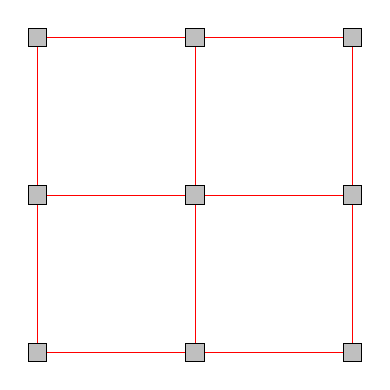
\begin{tikzpicture}
  \foreach \i in {0, 2, 4} {
    \draw[very thin, color = red] (0,\i) -- (4,\i);
    \draw[very thin, color = red] (\i,0) -- (\i,4);
  }
  \foreach \i in {0, 2, 4} {
      \foreach \j in {0, 2, 4} {
        \node[rectangle, fill = lightgray, draw=black] at (\i,\j) {};
      }
    }
  \end{tikzpicture}

\end{document}